\setmainfont{Noto Serif}
\setsansfont{Noto Sans}
\setmonofont{Noto Sans Mono}
\setstretch{1.35}
\hyphenation{ма-те-ма-ти-ка вос-ста-нав-ли-вать}


\section{Специальные хюккелевские системы}

1С. Определите основной терм $\pi$-системы циклобутадиена.
\par
2. Определите число разрешенных электрических дипольных переходов в~линейном радикале с $n$ центрами. Сколько разрешенных переходов имеют различную энергию?
\par
3С. Определите энергию высшей занятой молекулярной орбитали циклической системы с $n$ центрами ($n = 4k$, $n = 4k + 2$) при введении одного индуктивного заместителя $-\text{CH}_3$ группы.
\par
\begin{wrapfigure}{r}{45mm} %this figure will be at the right
    \centering
    \vspace{-4mm}
    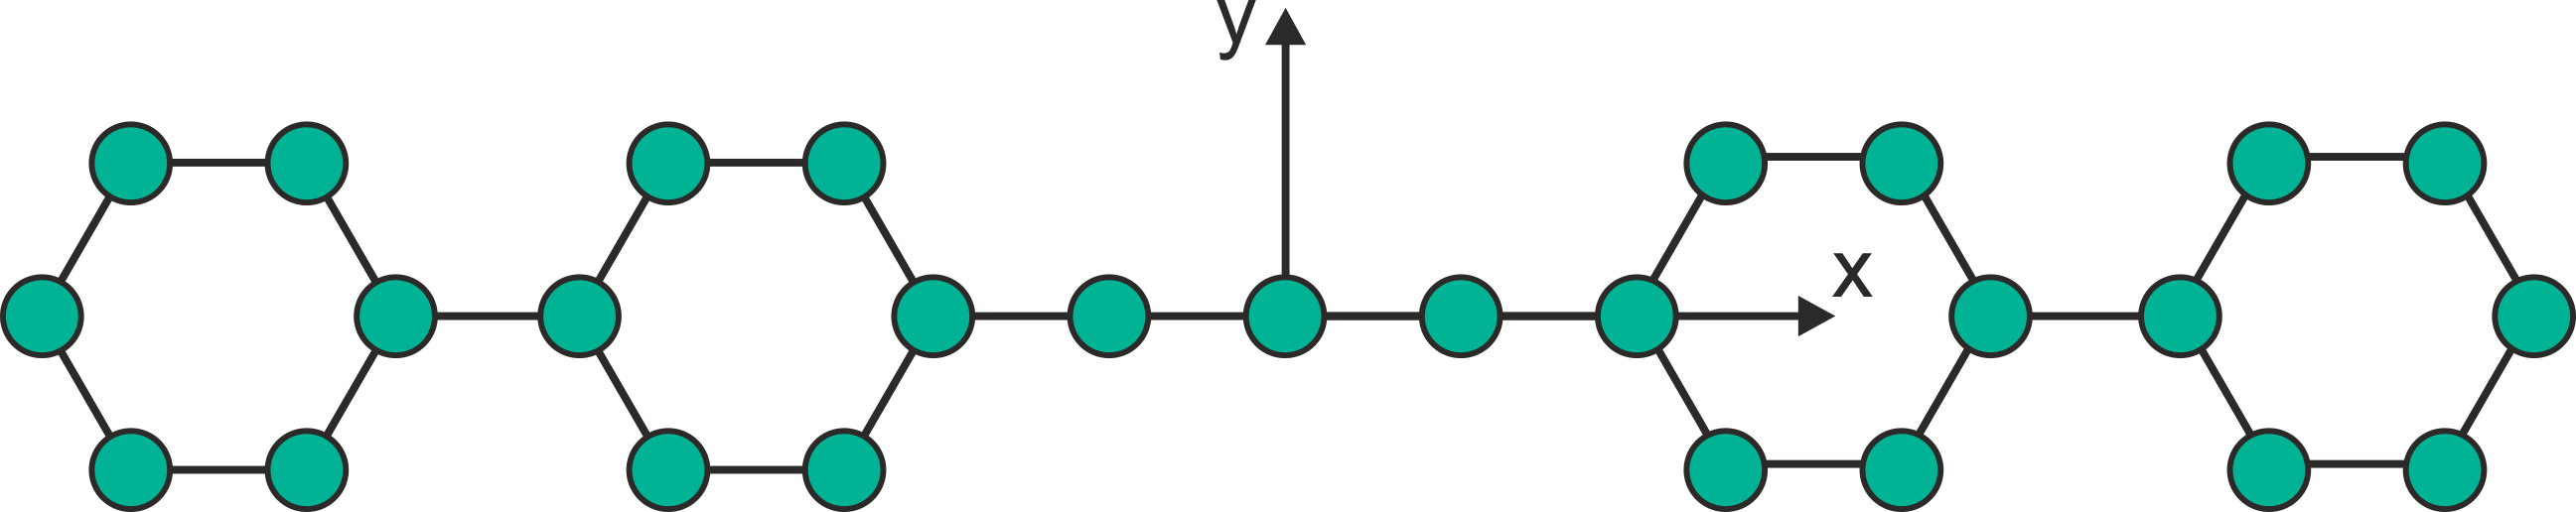
\includegraphics[width=45mm]{images/Fig_1_8_4.png}
    \vspace{-6mm}
\end{wrapfigure}
4С. Определите поляризацию электрического дипольного перехода между молекулярной орбиталью неспаренного электрона и~разрыхляющей молекулярной орбиталью с самой большой энергией для хюккелевской системы, изображенной на рисунке, в базисе $2p_z$ орбиталей.
\par
5. Используя метод Хюккеля качественно опишите электронное строение бесконечной линейной $\pi$-системы. Чему равно расстояние между энергетическими уровнями с максимальной и минимальной энергией?
\par
\begin{wrapfigure}{r}{30mm} %this figure will be at the right
    \centering
    \vspace{-7mm}
    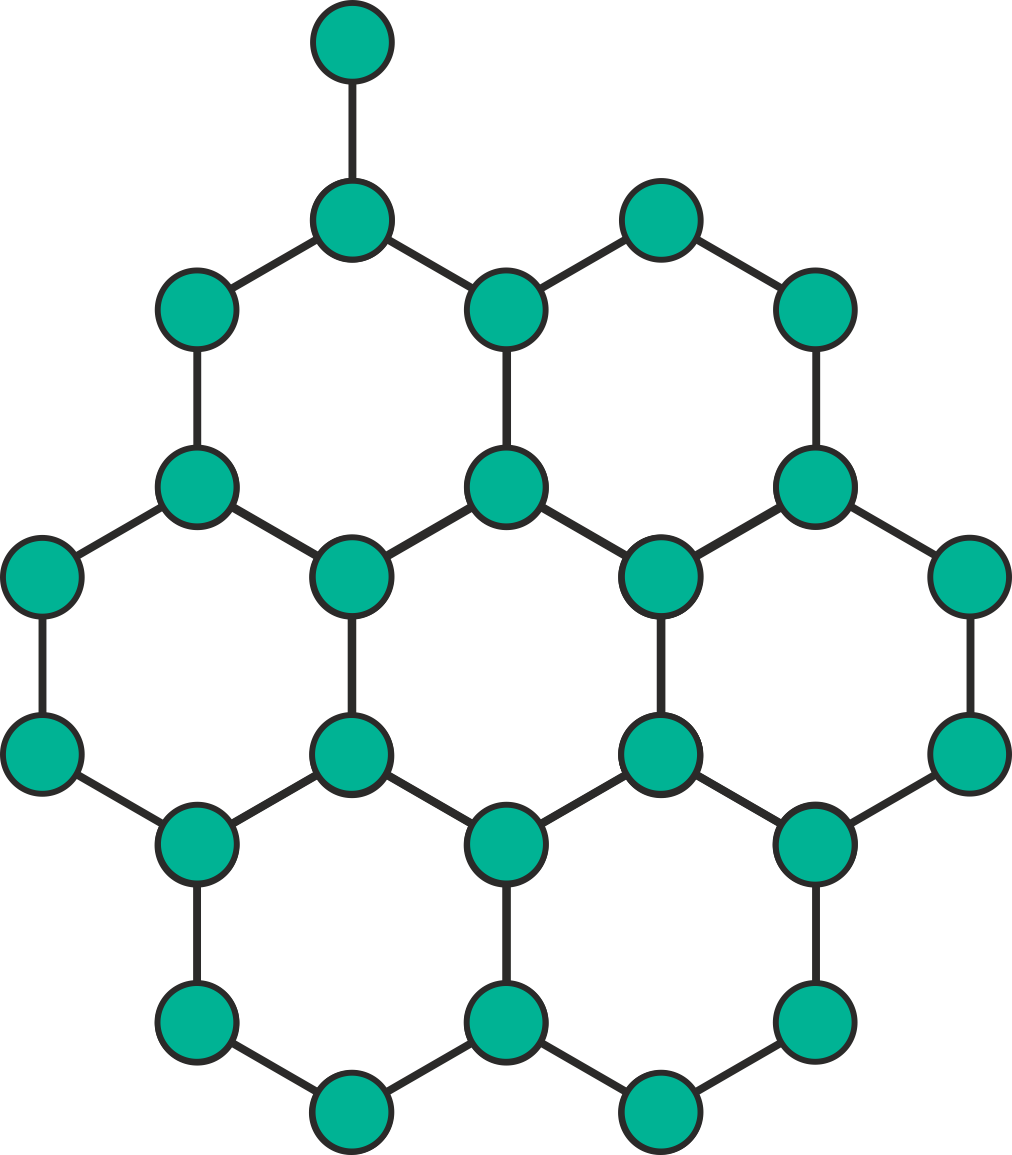
\includegraphics[width=17mm]{images/Fig_1_8_6.png}
    \vspace{-8mm}
\end{wrapfigure}
6С. Определите распределение спиновой плотности для $\pi$-системы, изображенной на рисунке справа. 
\par
7. Определите порядок $\pi$-связи между соседними центрами в~циклической системе с $n= 4k + 2$ центрами.
\par
8. Можно ли с помощью спектра поглощения определить квадратную или прямоугольную геометрию имеет $\pi$-система циклобутадиена? Все резонансные интегралы считать одинаковыми.
\par
9. Определить, какая из трех структур: (1) линейная, (2) угловая, (3) циклическая более устойчива для частиц $\text{H}_3$, $\text{H}_3^+$, $\text{H}_3^-$. В каждом случае определить распределение спиновой плотности и порядок связи.
\par
\begin{wrapfigure}{r}{36mm} %this figure will be at the right
    \centering
    \vspace{2mm}
    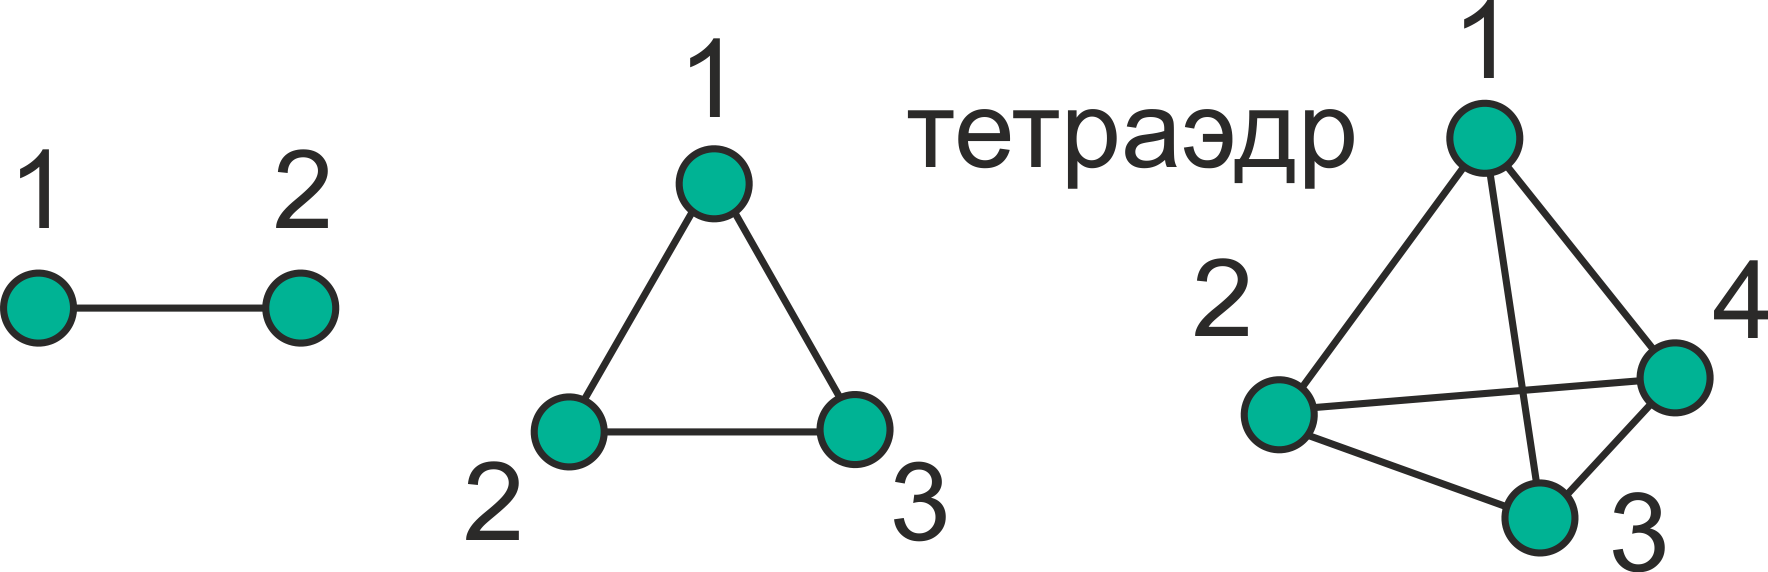
\includegraphics[width=34mm]{images/Fig_1_8_11.png}
    \vspace{-1mm}
\end{wrapfigure}
10К. Помимо циклических и альтернантных, к системам специального типа относятся также полносвязанные хюккелевcкие системы, в которых каждый центр связан с каждым. Три простейших примера таких систем изображены на рисунке. Используя приведенные примеры, экстраполируйте полученный для них ответ и~изобразите схему энергетических уровней для полносвязанной системы с~$n$~центрами. Определите также полную электронную энергию ее $\pi$-системы.
\par
\begin{wrapfigure}{r}{36mm} %this figure will be at the right
    \centering
    \vspace{-7.4ex}
    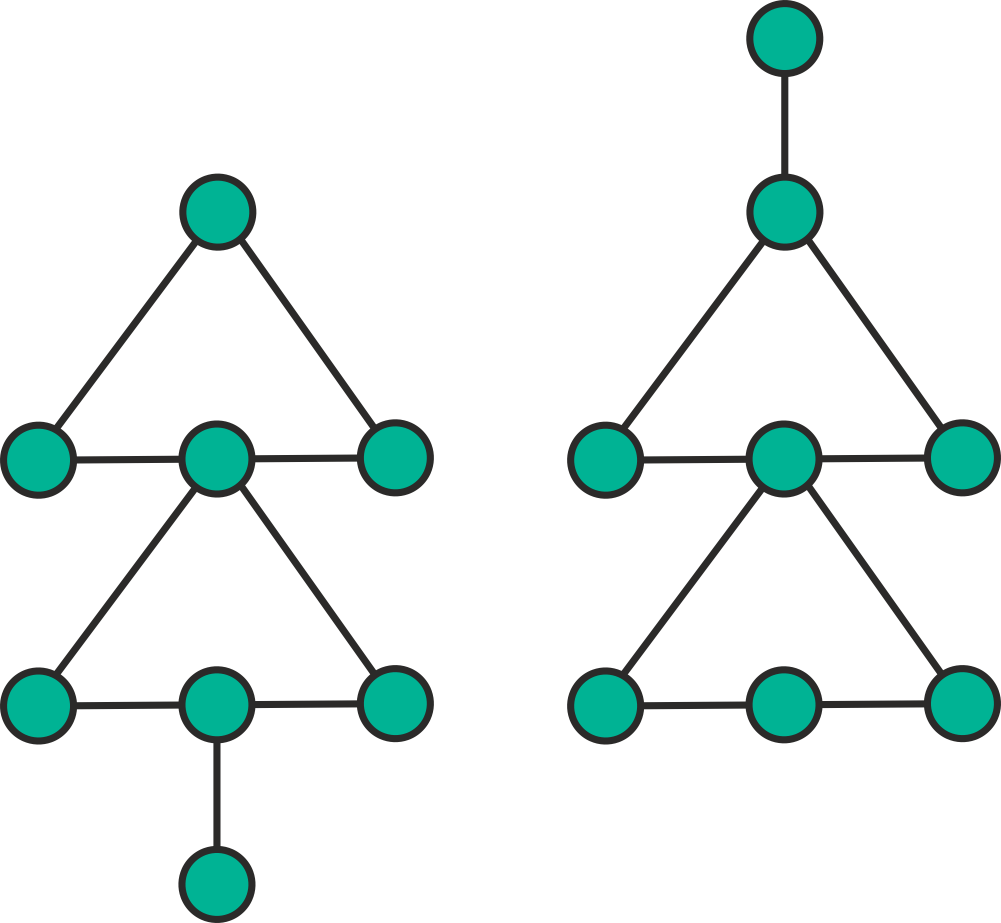
\includegraphics[width=19mm]{images/Fig_1_8_9.png}
    \vspace{-3ex}
\end{wrapfigure}
11. Определить распределение спиновой плотности в радикале, который имеет строение елочки. Рассмотрите два случая, изображенные на рисунке: (1)~елочка с ножкой, считая при этом, что резонансный интеграл с~самым нижним центром елочки равен $\sqrt{2}\beta$, (2) елочка со~звездочкой.
\par